\section{Compact-evidence annotation and mask selection}
\label{app:annotation-protocol}

The evaluation uses image--question examples whose short answer can be supported by a human-localizable image region. Each example records the image, question, fixed short-answer target, and an answer-bearing evidence mask. Annotators mark the smallest visible region that directly supports the answer; when visually separable context is necessary, a broader union mask is also retained. Examples with diffuse scene-level evidence, visually underspecified support, or an unalignable answer target do not enter the compact-evidence comparisons. The expanded regional evaluation contains 61 examples. A separate 52-example evaluation was selected and annotated without using previous model results.

\begin{figure}[!htbp]
    \centering
    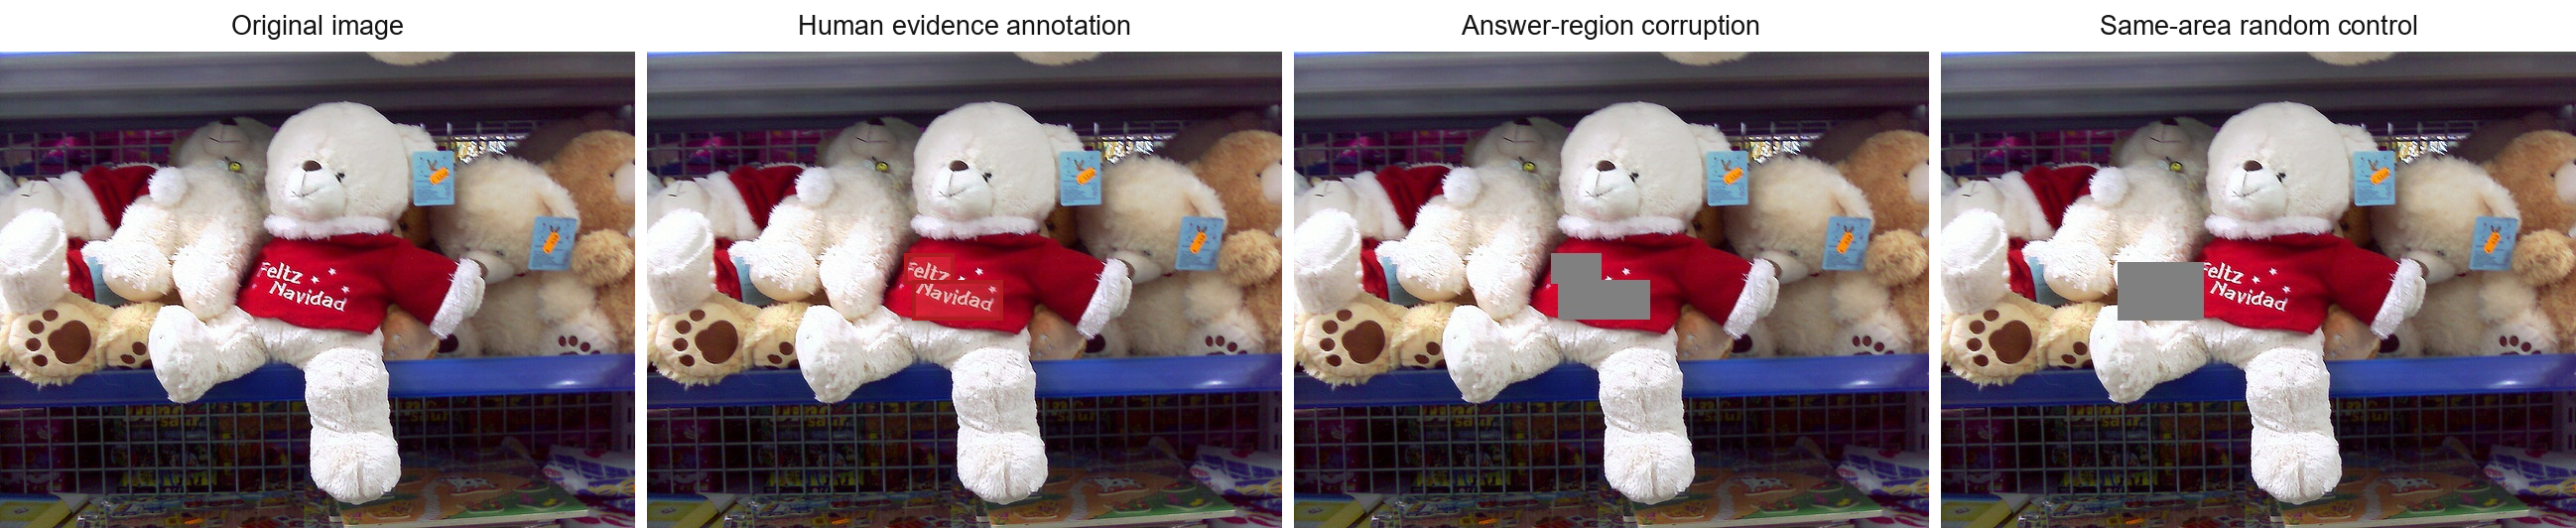
\includegraphics[width=\linewidth]{figures/okvqa_val_4739195_input_control_panel.png}
    \caption{\textbf{Example input, evidence annotation, and matched corruption.} For ``What language is the sign on the bear in?'' the target answer is ``Spanish.'' The panels show the original image, human annotation, gray answer-region corruption, and a same-area random corruption. This image illustrates mask construction; aggregate answer-score and intervention results are reported separately.}
    \label{fig:mask-annotation-example}
\end{figure}

The later full-hidden confirmation uses a different pool of 61 candidate masks. Following GPT-assisted pre-annotation, a human reviewed each mask without seeing model predictions or intervention results. One mask was rejected and the 60 accepted examples were evaluated with the interface and decision rule already frozen. This result-blind review is separate from the independently selected 52-example regional evaluation. The annotation workflow is single-pass, so no independent inter-annotator agreement estimate is available.
